\documentclass[25pt, a0paper, portrait, margin=0mm, innermargin=15mm, blockverticalspace=15mm, colspace=15mm, subcolspace=8mm]{tikzposter}

\usepackage[utf8]{inputenc}
\usepackage{amsmath}
\usepackage{amsfonts}
\usepackage{amssymb}
\usepackage{graphicx}
\usepackage{booktabs}
\usepackage{array}
\usepackage{multirow}
\usepackage{xcolor}
\usepackage{tikz}
\usetikzlibrary{calc}

% Define colors
\definecolor{darkblue}{RGB}{0,51,102}
\definecolor{lightblue}{RGB}{102,153,204}
\definecolor{accent}{RGB}{204,102,0}
\definecolor{lightgray}{RGB}{248,248,248}
\definecolor{clearbg}{RGB}{252,252,252}

% Custom color style with clearer background
\definecolorstyle{ClearStyle}{
    \colorlet{colorOne}{darkblue}
    \colorlet{colorTwo}{lightblue}
    \colorlet{colorThree}{accent}
}{
    % Background Colors
    \colorlet{backgroundcolor}{clearbg}
    \colorlet{framecolor}{darkblue}
    % Title Colors
    \colorlet{titlefgcolor}{white}
    \colorlet{titlebgcolor}{darkblue}
    % Block Colors
    \colorlet{blocktitlebgcolor}{lightblue}
    \colorlet{blocktitlefgcolor}{white}
    \colorlet{blockbodybgcolor}{white}
    \colorlet{blockbodyfgcolor}{black}
    % Innerblock Colors
    \colorlet{innerblocktitlebgcolor}{lightgray}
    \colorlet{innerblocktitlefgcolor}{black}
    \colorlet{innerblockbodybgcolor}{white}
    \colorlet{innerblockbodyfgcolor}{black}
    % Note colors
    \colorlet{notefgcolor}{black}
    \colorlet{notebgcolor}{lightgray}
    \colorlet{notefrcolor}{lightgray}
}
\definebackgroundstyle{ClearGradient}{
    \fill[top color=clearbg, bottom color=lightblue!20] 
    (bottomleft) rectangle (topright);
}

\usecolorstyle{ClearStyle}
\usebackgroundstyle{ClearGradient}

% Set poster theme with custom colors
\usetheme{Default}

% Standard title setup
\title{\Huge \textbf{Data Driven Derivative-based Regularization for Regression}}
\author{\Large Enrico Lopedoto$^*$, Kizito Salako$^*$, Maksim Shekhunov$^\dagger$, Vitaly Aksenov$^*$, Tillman Weyde$^*$}
\institute{\large $^*$City St George's University of London, UK \quad $^\dagger$ITMO University, St Petersburg, Russia}

\begin{document}

% Use standard maketitle first
\maketitle


\begin{columns}
    \column{0.33}
    
    \block{Introduction}{
        \textbf{Problem:} Traditional regularization methods (L1, L2, Dropout) only consider model parameters, ignoring characteristics of the target function that can be inferred from training data.
        
        \vspace{0.5cm}
        \textbf{Solution:} We propose \textbf{DLoss}, a novel regularization method that:
        \begin{itemize}
            \item Penalizes differences between model derivatives and estimated data derivatives
            \item Aligns the model to data in terms of both target values AND derivatives
            \item Is applicable to any model where loss functions can be specified
        \end{itemize}
        
        \vspace{0.5cm}
        \textbf{Key Innovation:} Using directional derivatives estimated from training data to guide model learning.
    }
    
    \block{Method Overview}{
        \begin{center}
            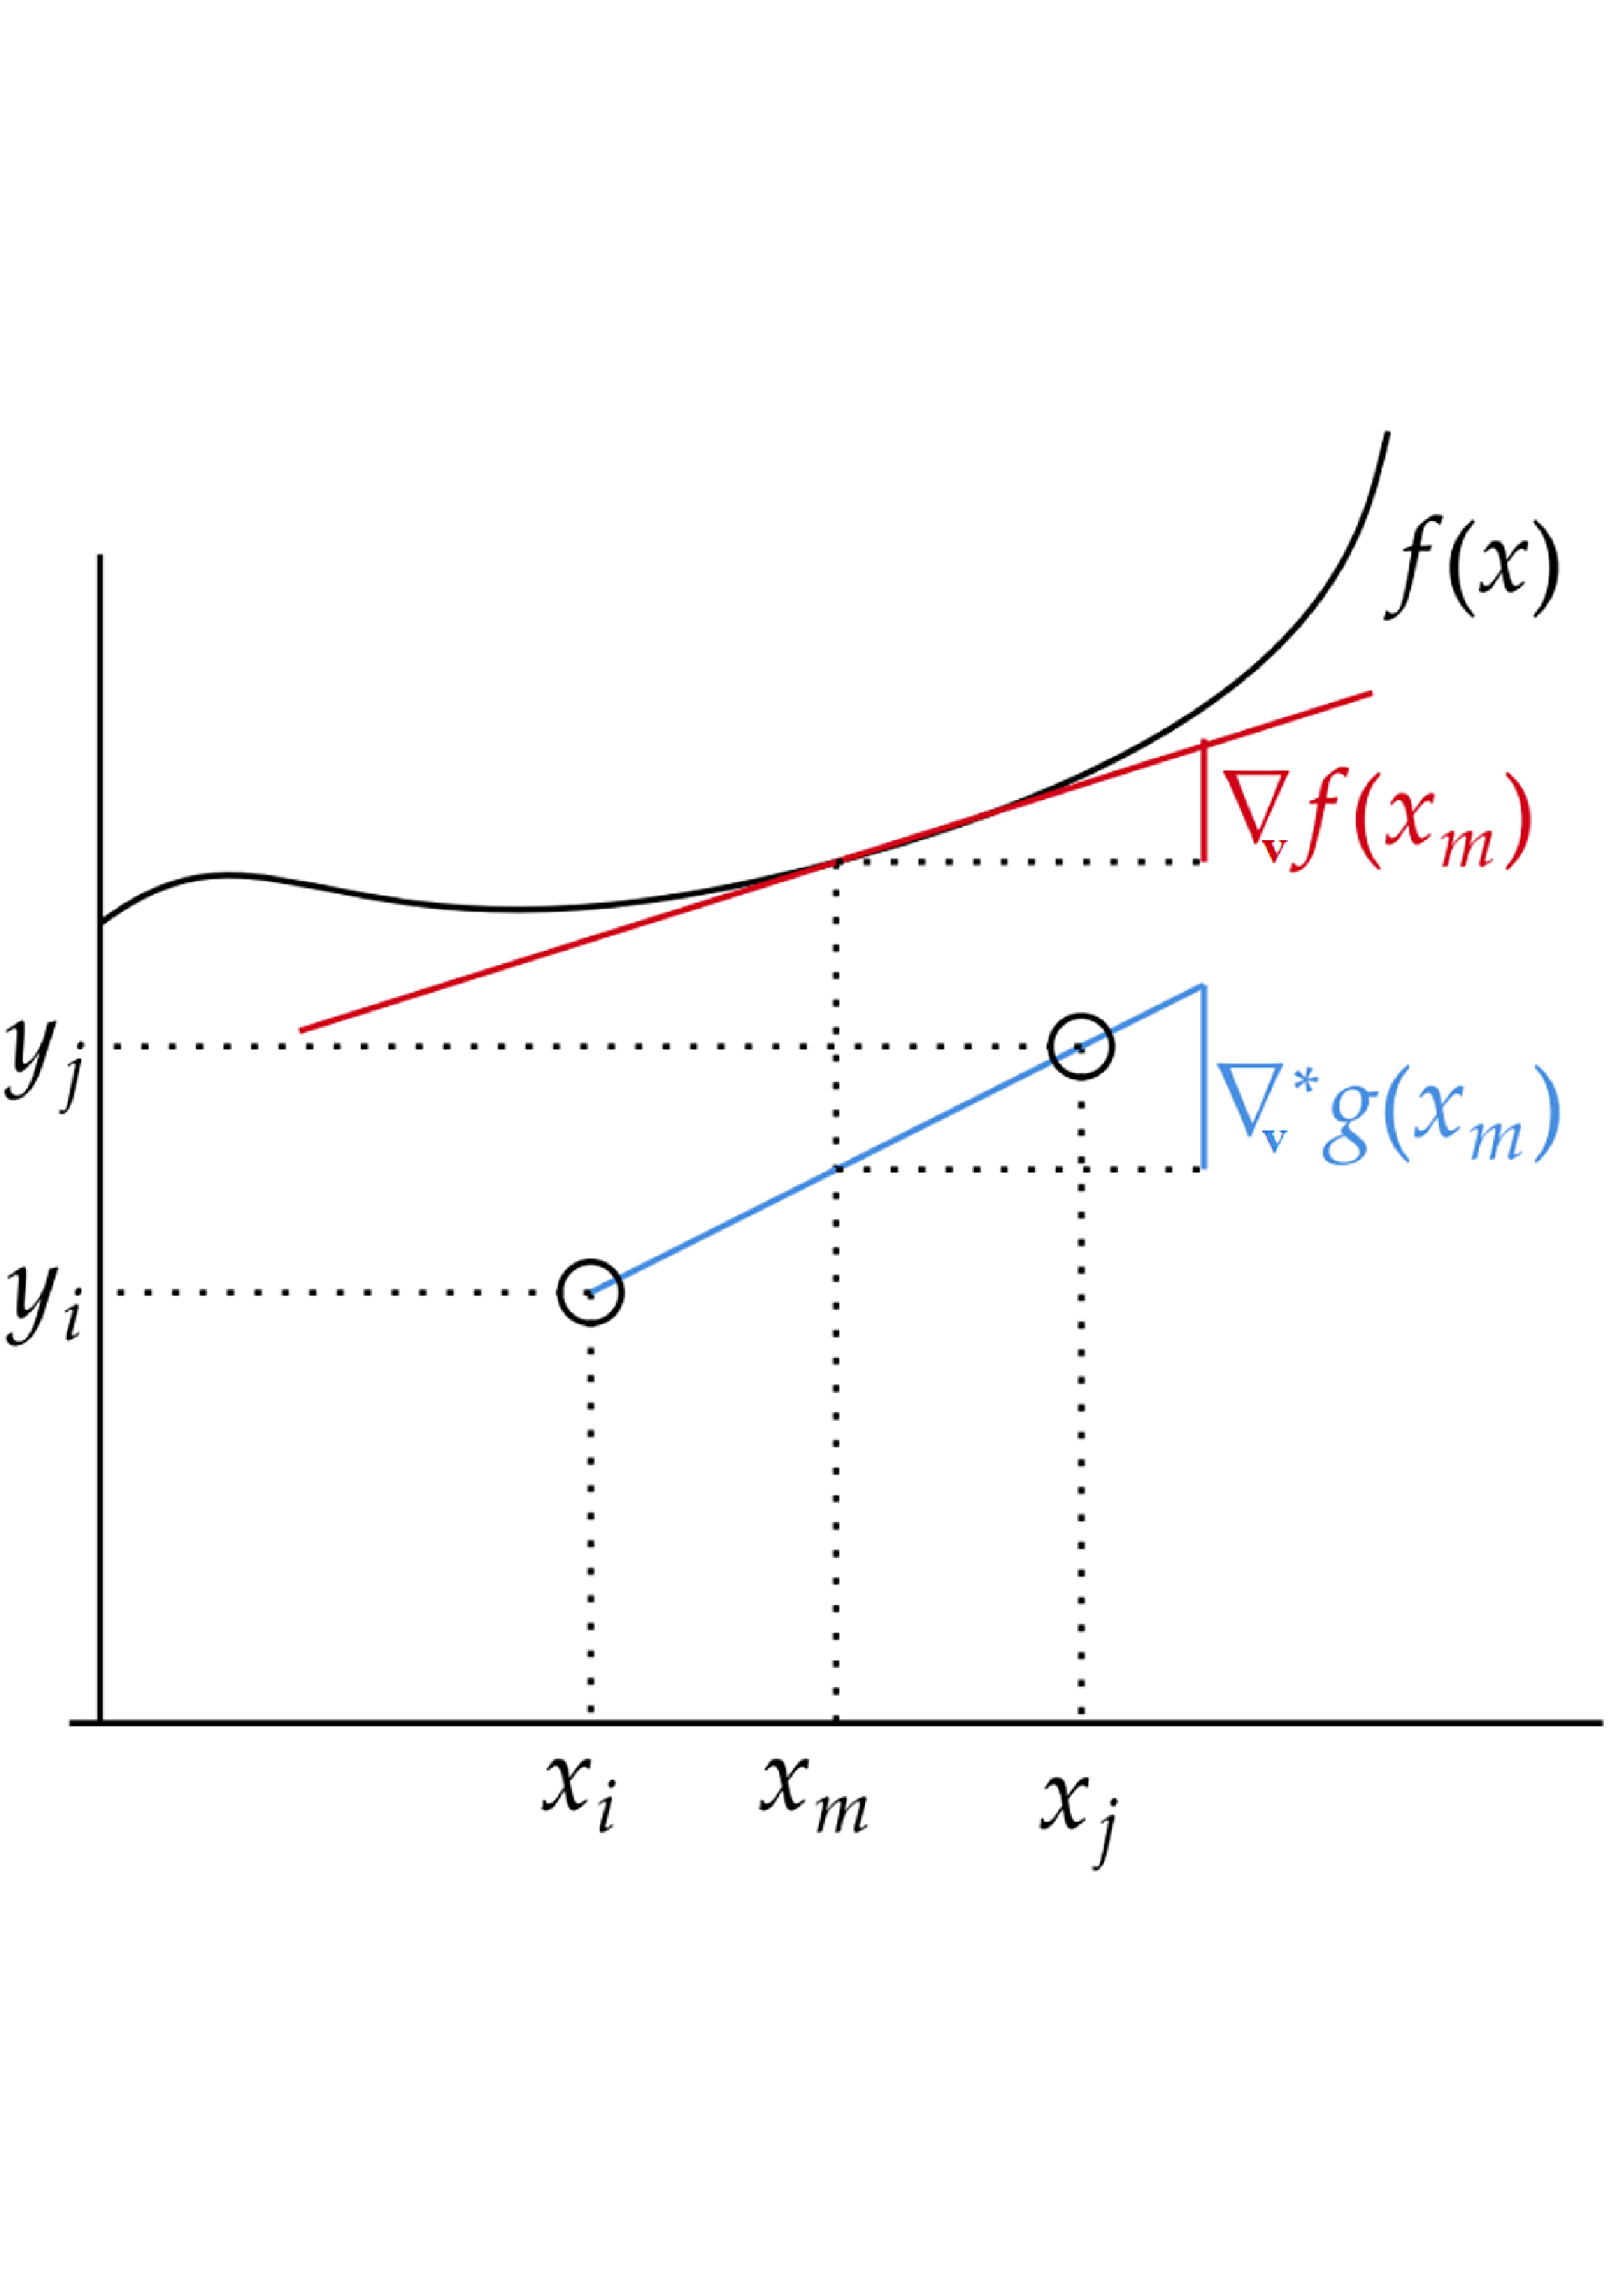
\includegraphics[width=1\linewidth]{diag2.pdf}
        \end{center}
        
        For a 2-tuple of data points $((x_i, y_i), (x_j, y_j))$:
        \begin{itemize}
            \item Calculate midpoint: $x_m = \frac{x_i + x_j}{2}$
            \item Difference vector: $v = x_j - x_i$
            \item Data derivative: $\nabla^*_v g(x_m) = \frac{y_j - y_i}{\|v\|_2}$
            \item Model derivative: $\nabla^\diamond_v f(x_m)$ (analytical or numerical)
        \end{itemize}
        
        \textbf{Goal:} Make model and data derivatives align (parallel slopes).
    }
    
    \block{DLoss Formulation}{
        \textbf{Derivative Difference:}
        $$dd(x) = \nabla^\diamond_v f(x) - \nabla^*_v g(x)$$
        
        \textbf{DLoss Regularizer:}
        $$\text{DLoss} = \frac{1}{|S|} \sum_{s \in S} dd(x^s_m)^2$$
        
        \textbf{Total Loss:}
        $$L = \theta_D \cdot \text{DLoss} + \text{MSE}$$
        
        where $S$ is the set of all selected tuples and $\theta_D$ is the weighting coefficient.
        
        \vspace{0.5cm}
        \textbf{Model Derivative (Numerical):}
        $$\nabla^\diamond_v f(x) = \frac{f(x + \epsilon\tilde{v}) - f(x - \epsilon\tilde{v})}{2\epsilon}$$
        where $\tilde{v} = \frac{v}{\|v\|_2}$ and $\epsilon = 0.001$.
    }
    
    \column{0.33}
    
    \block{Tuple Selection Strategies}{
        
         \begin{center}
            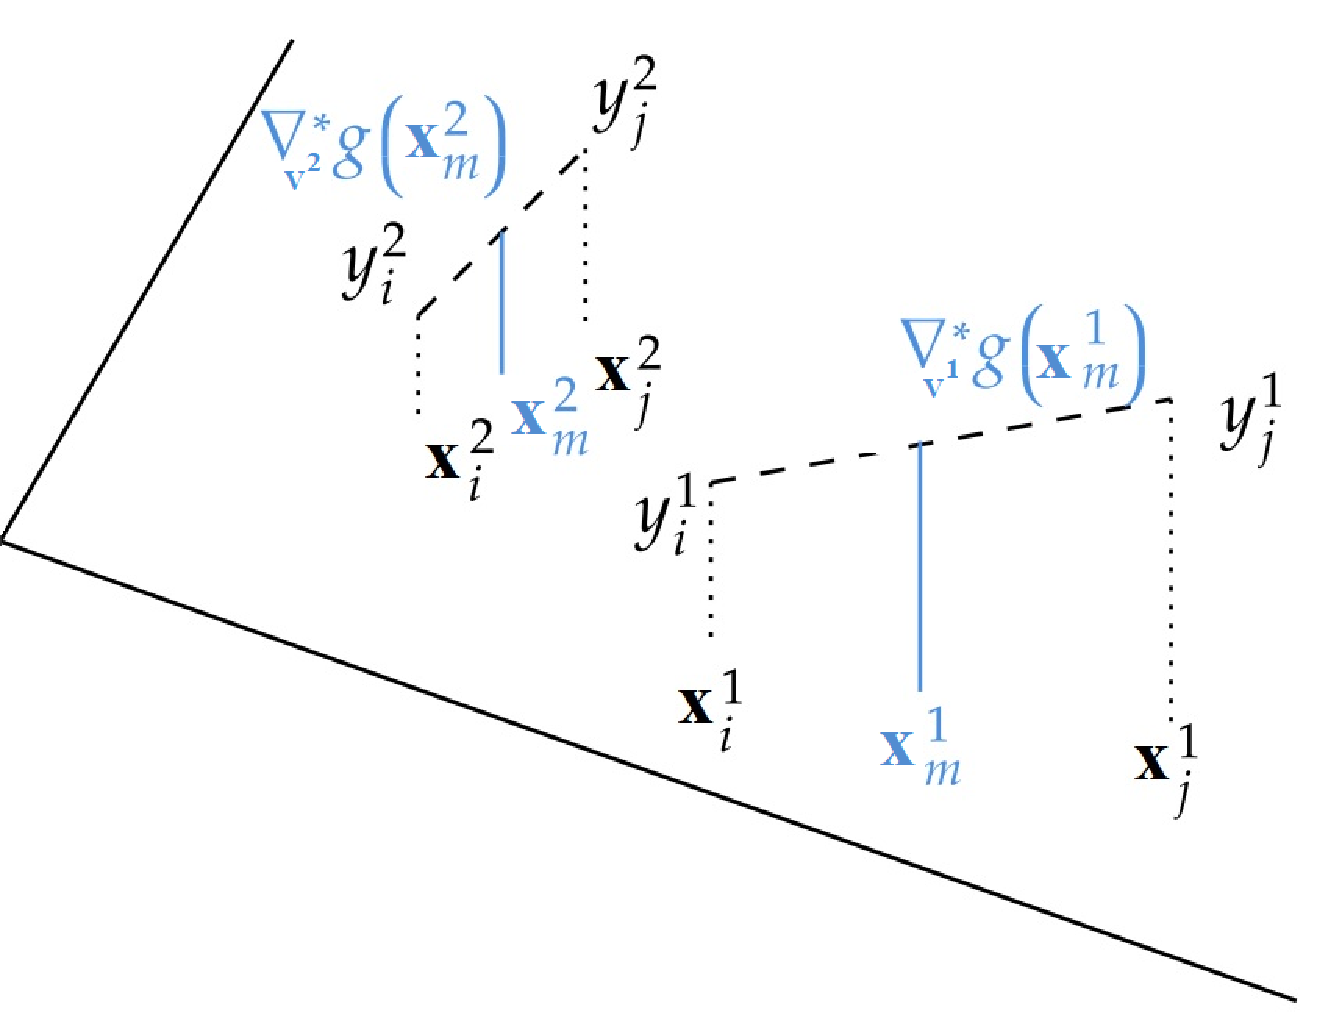
\includegraphics[width=1\linewidth]{diag1.pdf}
        \end{center}
        \textbf{Two approaches for selecting data point pairs:}
        
        \vspace{0.3cm}
        \textbf{1. Nearest Neighbor Selection (DLNN):}
        \begin{itemize}
            \item For each training point $(x_i, y_i)$, select $l$ nearest neighbors
            \item Uses efficient KD-tree algorithm
            \item Approximates derivatives using local information
            \item Time complexity: $O(nl + n\log n)$
        \end{itemize}
        
        \vspace{0.3cm}
        \textbf{2. Random Selection (DLRND):}
        \begin{itemize}
            \item For each training point, randomly select $l$ other points
            \item Less sensitive to noise (larger distances)
            \item Lower computational complexity: $O(nl)$
            \item Trade-off: less accurate derivative estimates
        \end{itemize}
    }
    
    \block{Experimental Setup}{
        \textbf{Model Architecture:}
        \begin{itemize}
            \item Feed-forward neural network
            \item Single hidden layer with 64 neurons
            \item ReLU activation function
            \item Adam optimizer
        \end{itemize}
        
        \vspace{0.3cm}
        \textbf{Datasets:}
        \begin{itemize}
            \item \textbf{Real data:} Wine, Cancer, Diabetes, Modechoice, Anes96
            \item \textbf{Synthetic data:} F1, Regression1, Regression10, Sparse-uncorrelated, Swiss Roll
        \end{itemize}
        
        \vspace{0.3cm}
        \textbf{Comparison Methods:}
        \begin{itemize}
            \item STD: No regularization
            \item L2: L2 weight decay
            \item DO: Dropout
            \item DLRND: DLoss with random selection
            \item DLNN: DLoss with nearest neighbor selection
        \end{itemize}
        
        \vspace{0.3cm}
        \textbf{Evaluation:} 5-fold cross-validation, 250 epochs, grid search over hyperparameters
    }
    
    \block{Key Findings}{
        \begin{itemize}
            \item \textbf{DLNN achieves best overall performance} with average rank 1.7
            \item \textbf{Nearest neighbor selection outperforms random selection} for derivative estimation
            \item \textbf{DLoss weight $\theta_D$ is higher for synthetic data} (noise-free) than real data
            \item \textbf{Computational overhead is moderate} - roughly 2-3x training time
            \item \textbf{All regularization methods significantly better than no regularization}
        \end{itemize}
    }
    
    
    \column{0.33}
    
    \block{Results \& Performance Analysis}{
        \textbf{Method Rankings by Validation MSE:}
        \begin{center}
        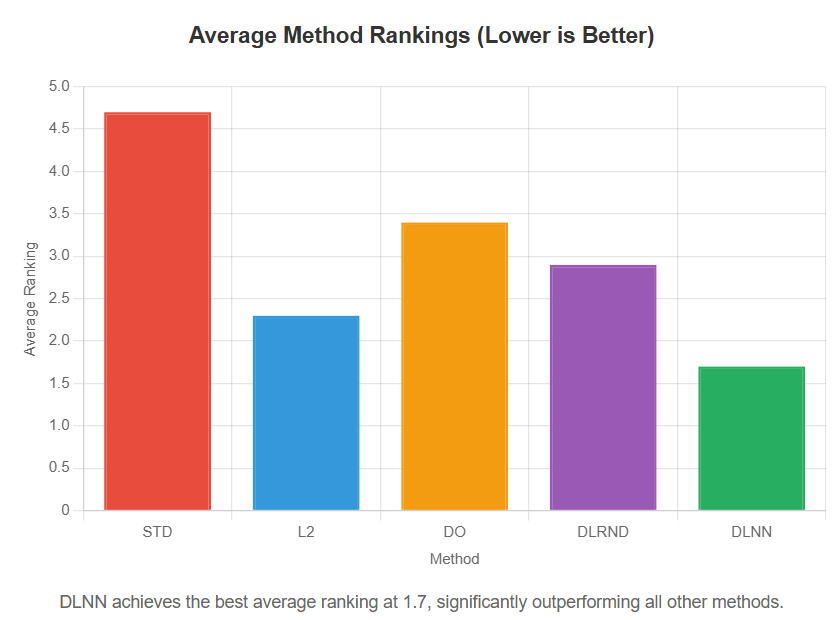
\includegraphics[width=1\linewidth]{ranking_chart.png}
        \end{center}
        
        \vspace{0.3cm}
        \textbf{Mean Reciprocal Rank (MRR):}
        \begin{center}
        \begin{tabular}{lc}
            \toprule
            \textbf{Method} & \textbf{MRR} \\
            \midrule
            \textbf{DLNN} & \textbf{0.716} \\
            L2 & 0.570 \\
            DLRND & 0.408 \\
            DO & 0.373 \\
            STD & 0.215 \\
            \bottomrule
        \end{tabular}
        \end{center}
        
        \vspace{0.3cm}
        \textbf{Computational Efficiency:}
        \begin{center}
        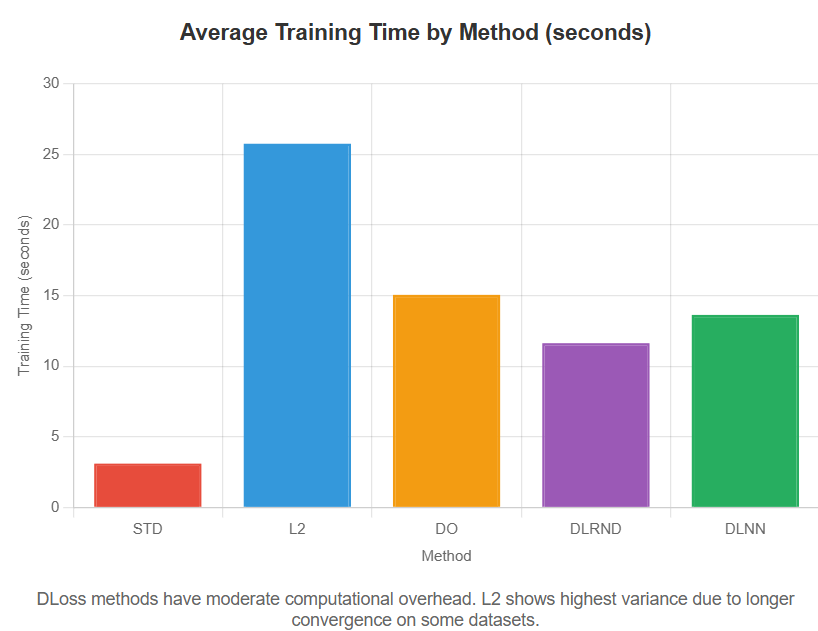
\includegraphics[width=1\linewidth]{time.png}
        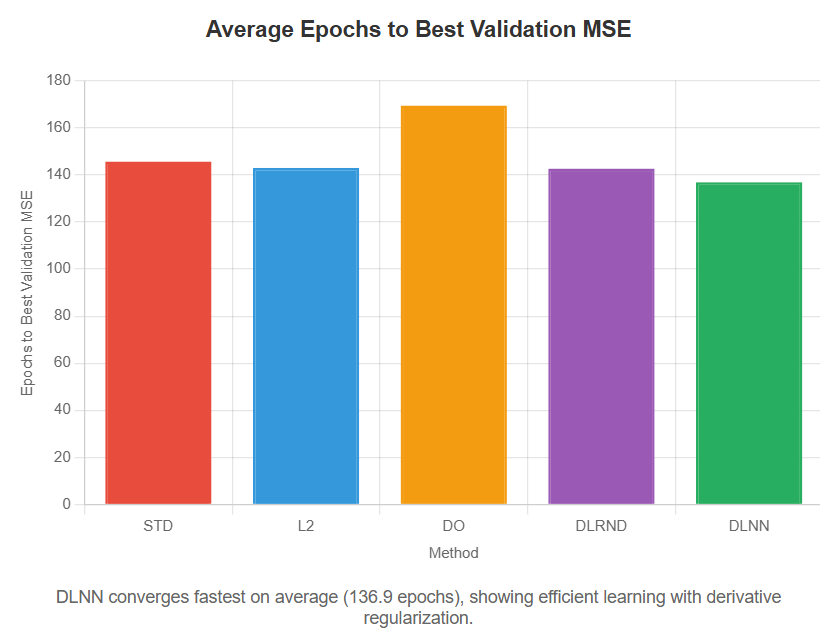
\includegraphics[width=1\linewidth]{epoch.png}

        \end{center}
        
        \vspace{0.3cm}
        \textbf{Statistical Significance:}
        DLNN significantly outperforms DLRND, DO, and STD (Wilcoxon signed rank test, p < 0.05).
    }
    
    \block{Conclusions \& Future Work}{
        \textbf{Contributions:}
        \begin{itemize}
            \item Novel data-driven regularization using derivatives
            \item Applicable to any differentiable model
            \item Demonstrated improvement over standard methods
        \end{itemize}
        
        \vspace{0.3cm}
        \textbf{Future Directions:}
        \begin{itemize}
            \item Extension to classification problems
            \item Combination with other regularization methods
            \item Testing on larger datasets and deeper networks
            \item Analytical gradient computation to reduce cost
        \end{itemize}
        
        \vspace{0.5cm}
        \textbf{Code Available:} \texttt{https://github.com/EnricoLope}
    }

\end{columns}

\end{document}